\documentclass[]{tufte-handout}

% ams
\usepackage{amssymb,amsmath}

\usepackage{ifxetex,ifluatex}
\usepackage{fixltx2e} % provides \textsubscript
\ifnum 0\ifxetex 1\fi\ifluatex 1\fi=0 % if pdftex
  \usepackage[T1]{fontenc}
  \usepackage[utf8]{inputenc}
\else % if luatex or xelatex
  \makeatletter
  \@ifpackageloaded{fontspec}{}{\usepackage{fontspec}}
  \makeatother
  \defaultfontfeatures{Ligatures=TeX,Scale=MatchLowercase}
  \makeatletter
  \@ifpackageloaded{soul}{
     \renewcommand\allcapsspacing[1]{{\addfontfeature{LetterSpace=15}#1}}
     \renewcommand\smallcapsspacing[1]{{\addfontfeature{LetterSpace=10}#1}}
   }{}
  \makeatother

\fi

% graphix
\usepackage{graphicx}
\setkeys{Gin}{width=\linewidth,totalheight=\textheight,keepaspectratio}

% booktabs
\usepackage{booktabs}

% url
\usepackage{url}

% hyperref
\usepackage{hyperref}

% units.
\usepackage{units}


\setcounter{secnumdepth}{-1}

% citations

% pandoc syntax highlighting

% longtable

% multiplecol
\usepackage{multicol}

% strikeout
\usepackage[normalem]{ulem}

% morefloats
\usepackage{morefloats}


% tightlist macro required by pandoc >= 1.14
\providecommand{\tightlist}{%
  \setlength{\itemsep}{0pt}\setlength{\parskip}{0pt}}

% title / author / date
\title{WFU Update - \href{mailto:LTC@Duke}{\nolinkurl{LTC@Duke}}}
\author{Allen S. Brown}
\date{March 20th, 2019}


\begin{document}

\maketitle




\newthought{In preparation for} the Spring 2019 LTC meeting at Duke,
\href{https://is.wfu.edu/academic-technologies/about/}{Hannah Inzko},
\href{https://oe.wfu.edu/about/}{Brenda Knox},
\href{https://is.wfu.edu/academic-technologies/whats-news/wakerspace/}{Paul
Whitener}, \href{https://oe.wfu.edu/about/}{Allen Brown}, and
\href{https://is.wfu.edu/academic-technologies/about/}{Brianna
Derr}\footnote{You'll hear Brianna's voice on the introduction to the
  podcast. Many thanks to her for producing this pod.} gathered to
discuss what they're talking about on campus with regards to learning
technologies.

\emph{\href{https://prod.wp.cdn.aws.wfu.edu/sites/232/2019/03/LTC_update_pod.mp3}{LTC
Update Podcast}}\footnote{\href{https://prod.wp.cdn.aws.wfu.edu/sites/232/2019/03/LTC-Update-Pod-Edited.pdf}{Transcript}}

This offered a chance for Hannah and Brenda to still contribute to the
meeting despite their absences, and for Paul\footnote{\ldots{}and his
  work with the \href{https://twitter.com/WakerSpace}{Wakerspace},
  pictured below.} to introduce himself to the group.

\begin{marginfigure}
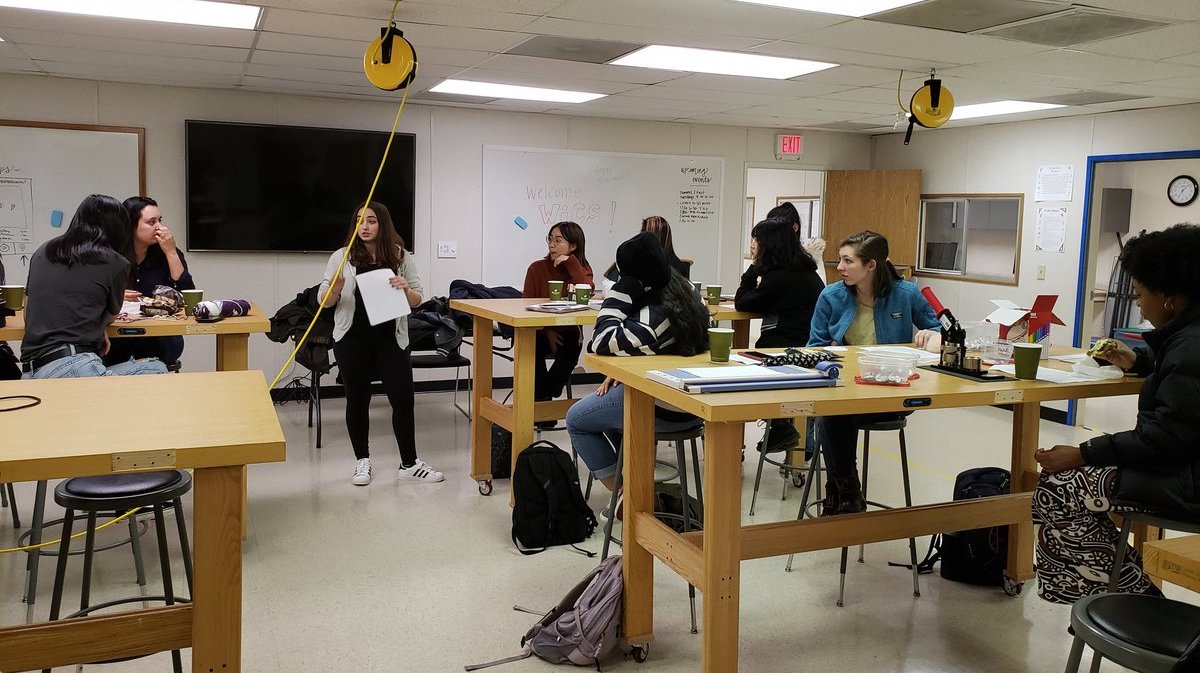
\includegraphics{images/wakerspace} \end{marginfigure}

We encourage you to listen to the pocast for an overview of things
happening at Wake, or continue reading below for further detail.

\section{Engaging Campus Communities}\label{engaging-campus-communities}

In recent years, Information Services (IS) and others involved in
Academic Technologies at Wake Forest have been redesigning the
structures that exist to engage the various communities and stakeholders
at Wake in a more sustainable manner.\footnote{I.e., less personality
  driven and more strucurally embedded.} IS governance has established
two types of groups -
\href{https://is.wfu.edu/group/initiative-teams/}{Initiative Teams} and
\href{https://is.wfu.edu/group/communities-of-interest/}{Communities of
Interest} - for addressing community needs and encouraging exploration.
Initiative teams are tasked with specific projects or services. While
several of these teams already existed on campus,\footnote{Such as the
  \href{https://is.wfu.edu/governance/learning-management-systems/}{LMS
  team}} the restructured governance has provided a more effective path
for communicating practices campus wide and establishing policy in areas
of cross-institutional interest. Initiative teams target both
administrative services\footnote{Including GDPR, Workday implementation,
  and room reservation management systems (i.e.~EMS)} and teaching and
learning efforts.\footnote{The
  \href{https://is.wfu.edu/governance/learning-spaces/}{Learning Spaces}
  team, for example.}

Communities of Interest engage similarly constructed groups in more
open-ended exploration. One example is the
\href{https://is.wfu.edu/governance/e-portfolio/}{ePortfolio CoI} which
shares best practices from ePortfolio implementations, researches
developments in the broader field, and provides feedback on the
selection and integration of these tools into programs. This community
is currently partnering with the
\href{https://leadershipandcharacter.wfu.edu/what-we-do/current-initiatives/}{President's
Commission on the First Year Experience} at Wake to identify whether and
how ePortfolios might be implemented in support of this program. Another
CoI, the Business Analytics and Informatics team, has adopted a new
licsensing structure for Microsoft Power BI on campus and is currently
rolling out this tool to support teams, programs, and schools in
collaborative, data-informed decision making. CoI's are typically open
to any faculty and staff at the university. Specific efforts are also
being made to involve students as regular participants in these groups

\begin{marginfigure}
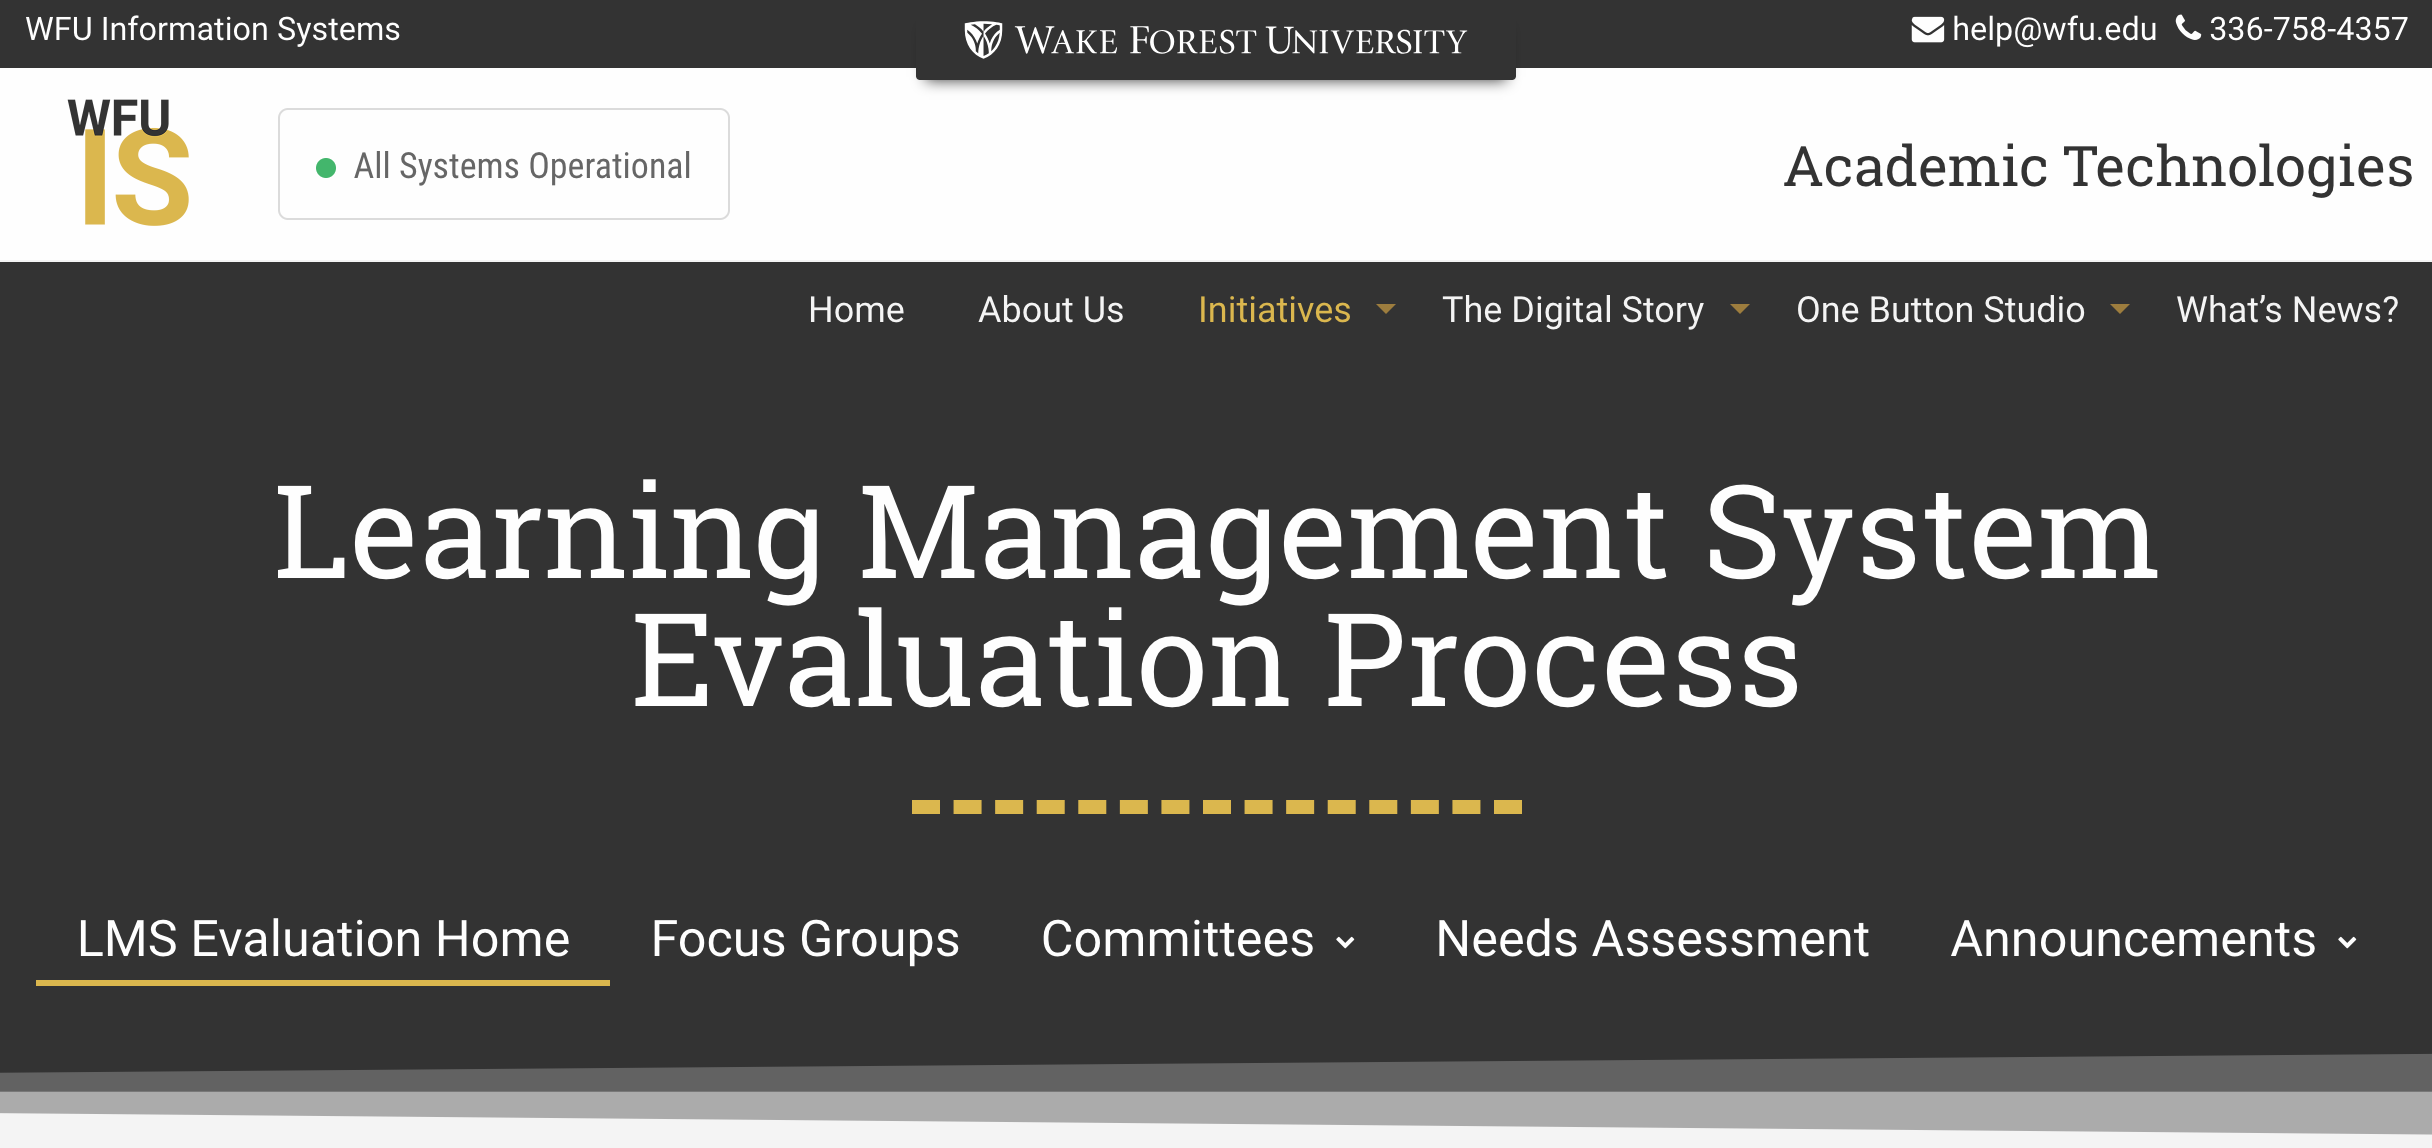
\includegraphics[width=33.78in]{images/lms_process} \end{marginfigure}

\subsection{LMS Evaluation}\label{lms-evaluation}

One project that extends beyond these smaller teams is the current
\href{https://is.wfu.edu/academic-technologies/lms-review/}{LMS
Evaluation}, overseen by the Director of Academic Technology. The
process, which has been documented publicly for the community, began
with a series of conversations that led to structured focus groups (with
staff, faculty, and students) and a needs assessment survey delivered to
the campus community. The focus groups and survey feedback was
incorporated into a formal RFP. Proposals received from vendors were
evaluated by a representational committee. This committee selected two
LMSs to invite for on-campus presentations during the week of March
25th. Representatives for both Sakai and Canvas\footnote{Sakai is the
  University's current LMS, and will be represented on campus by
  Longsight. Two online Masters programs currently use Canvas.} will
deliver a
\href{https://us18.campaign-archive.com/?e=\&u=bea1d79e7a99dd4ba1507c539\&id=dd32f72c28}{series
of demonstrations} open to the entire campus community. While this
effort will not preclude further explorations into
\href{https://er.educause.edu/articles/2017/7/the-ngdle-we-are-the-architects}{Next-Generation
Digital Learing Environments}, discusisons of NGDLEs have not been
centered in this process.\footnote{One current effort exploring NGDLEs
  on a smaller scale comes from librarian
  \href{https://zsr.wfu.edu/directory/kyle-denlinger/}{Kyle Denlinger},
  who is hosting his online course this spring without a traditional
  LMS.}

\subsection{Creative Exchanges}\label{creative-exchanges}

One effort to engage the broader campus community that is taking on a
more grassroots approach is a new foray into Creative Exchanges. Modeled
after aspects of \href{https://www.creativecommunities.group/}{Creative
Communities}, Creative Exchanges participants gather at monthly meetings
in which individuals across the WFU community (really anyone engaging in
``creative'' work, as they define it) meet to hear about creative work
from another community member, network with others in the group, and
explore potential collaborations (digital or otherwise). The first
gathering is scheduled for Monday, April 1st.

\begin{marginfigure}
\includegraphics{images/creatives} \end{marginfigure}

\section{Supporting Evidence Based Practices in Teaching and
Learning}\label{supporting-evidence-based-practices-in-teaching-and-learning}

A recurring topic in recent WFU updates at LTC has been the emerging
Teaching and Learning Collaborative.
\href{http://www.elizabethbarre.com/}{Betsy Barre} arrived as the new
Executive Director for the collaborative in May of 2018, and she has
been engaging the many campus partners throughout the current academic
year in establishing a clear vision for the future of the Collaborative.
While the vision for this group will likely be finalized in the coming
months, two items of note are already clear. First, the Offices of
Online Education and Academic Technology will continue to work in
partnership with the TLC but will not be joined in a single reporting
structure. And second, this new vision will center support for
evidence-based practices and scholarship on teaching and learning.

The TLC is currently nearing the end of its search for a postdoctoral
research associate. This new hire will be tasked with increasing the
Collaborative's capacity for internal program evaluation,
institution-level research, and the scholarship of teaching and
learning. This one-year position will include a mutual option for a
second year with the possibility for it to develop into a permanent
staff role. The Director is also working to implement a smoother path to
conducting educational research similar to current models established at
Duke, Carnegie Mellon, and Rice.\footnote{It looks like we will hear
  more from Duke on
  \href{https://mfeldstein.com/educational-research-irb-infrastructure/?elqTrackId=8f8d51420d244c22a9a0235548926b8d\&elq=e757e3a03c5b4112ae6267887dac73f8\&elqaid=22301\&elqat=1\&elqCampaignId=10980}{their
  work} in this area.} In addition to supporting and growing faculty
efforts in educational research, the center is also exploring strategies
for engaging the \href{https://ureca.wfu.edu/}{undergraduate} and
\href{https://tlc.wfu.edu/what-we-do/postdoc-ta-support/}{graduate
student} populations in more of this work as well.

\subsection{Learning Analytics}\label{learning-analytics}

A related area to educational research is the growing body of work on
learning analytics. While few individuals at Wake currently classify
their work as ``learning analytics,'' several current efforts overlap
with the field's working definitions.\footnote{\emph{The measurement,
  collection, analysis and reporting of data about, and with, learners
  and their contexts for purposes of understanding and optimizing
  learning and the environments in which learning occurs (SoLAR, 2011).}}
To that end, the TLC has established a series of exploratory efforts
this academic year designed to identify meaningful strategies for
supporting and encouraging individual and interdisciplinary efforts in
learning analytics-type work at an institutional level. While many
analytic tools might be used to promote this work, the TLC has chosen to
ground its work in R and R Studio with the hope that its open
availability and relatively accessible development environment will
encourage participation, promote interdisciplinary efforts, and develop
skills that students, staff, and faculty might continue to use in their
efforts beyond Wake.

The TLC and the Digital Humanities group at Wake have partnered to
facilitate a year-long \href{https://tlc.wfu.edu/r}{faculty learning
community} on Data Analysis in R for research and learning. While the
community's efforts have taken shape as the process evolved, a
significant amount of the progress has been documented on the
\href{https://wfu-tlc.github.io/sessions.html}{group's website}. In
addition to supporting and developing current participants, the
participants themselves are providing feedback to inform future efforts
targeted at faculty growth in this area. Another partnership has
involved a data scientist from Institutional Research to deliver two
workshop series open to faculty, staff, and graduate students.\footnote{Materials
  from the first workshop series (delivered in Fall 2018) are
  {[}available
  online{]}(\url{https://michaeldewittjr.com/introduction_to_r/lectures.html}.}
These workshops focus more explicitly on the development of technical
skills in R and R Studio while fostering community among practitioners
on campus. Particular interest from graduate students in these workshops
has prompted further discussions about incorporating instruction on SoTL
practices into the TLC's TA/PostDoc training. Additionally, since
learning analytics opens up several ethical and moral concerns around
practice, a third effort has begun to identify partners and stakeholders
at the university who might work together to develop a code of practice
(or similar policy)\footnote{One model for
  \href{https://www.csu.edu.au/__data/assets/pdf_file/0007/2160484/2016_CSU_LearningAnalyticsCodePractice.pdf}{such
  a code} and its development is available from Colorado State
  University} around learning analytics efforts here at Wake. Finally,
Allen Brown has been engaging with the broader learning analytics
community on behalf of the TLC in order to establish Wake Forest's
presence among the broader field while reporting back on existing wisdom
and practices from the community to further inform work on this
campus.\footnote{This includes attendance at IU's first
  \href{https://lasummit.indiana.edu/}{Learning Analytics Summit},
  \href{https://lak19.solaresearch.org}{LAK19}, contributions to
  \href{https://onlinelearningconsortium.org/olc-innovate-2019-session-page/?session=6720\&kwds=}{OLC
  Innovate}, and participation in Oregon State's new
  \href{https://ecampus.oregonstate.edu/research/opportunities/online-teaching-learning-research-seminars/}{eCampus
  Research Seminar}.}

\section{Additional Notes}\label{additional-notes}

\subsection{Video Management Platform}\label{video-management-platform}

Academic Technology is leading an effort to identify an institution wide
video management platform. While various schools and programs at Wake
provide their own platform to support classroom video, streaming, and
lecture capture, the VMP committee is reviewing proposals from four
vendors\footnote{Echo360, Kaltura, Panopto, \& WarpWire} with the goal
of identifying one platform that can best meet the needs of diverse
constituencies across the institution. The team has already reached out
to others in the LTC community and welcomes additional insight into
video management platforms hosted at other institutions.

\subsection{Digital Learning}\label{digital-learning}

The Office of Academic Technology have several additional projects of
note.\footnote{Learn more about Academic Technologies efforts at their
  \href{https://spark.adobe.com/page/356WBwoJHJCp2/}{Semester in Review
  site}} Brianna Derr, Manager of Advanced Learning Projects, is heading
up two new efforts at Wake. The Technology Consultant program supports
undergraduate student workers as part of the Academic Technology team.
This year there are four consultants who receive training and mentoring
as they complete unique digital projects or deliver workshops and
consultations to their peers. Their work helps to extend the digital
learning footprint at Wake while developing new student leaders.

\begin{marginfigure}
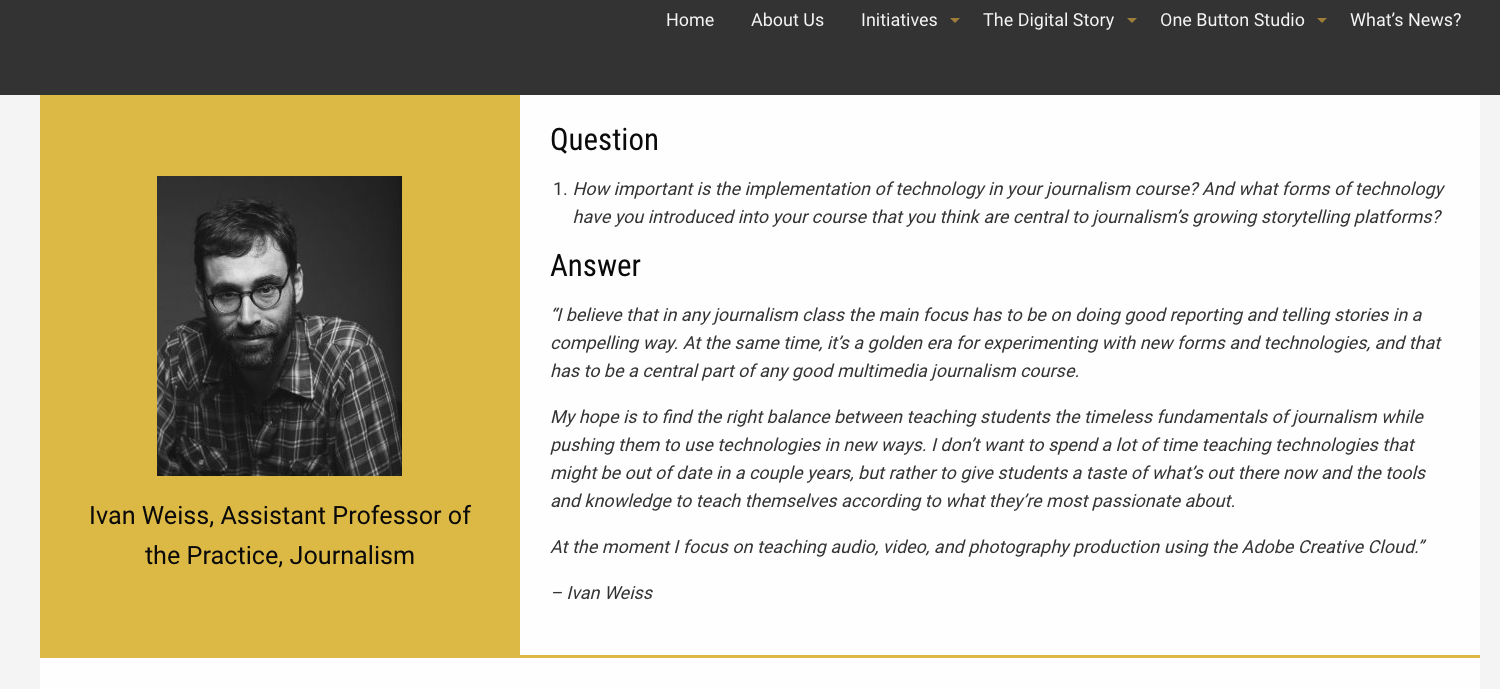
\includegraphics[width=20.83in]{images/weiss} \end{marginfigure}

This team is also highlighting some of the unique instructional projects
that faculty have implemented in their classes following individual
consultations. Ivan Weiss worked with Brianna to design a multimedia
storytelling assignment for students in a Journalism course. The
\href{https://is.wfu.edu/academic-technologies/story/journalism-multimedia-storytelling/}{Digital
Story page} includes an overview of the project, a showcase of student
work, and reflection from the instructor. The classroom project
overviews are supplemented by a
\href{https://is.wfu.edu/academic-technologies/podcasts/}{podcast
series} diving deeper into the faculty and their digital learning work.

\subsection{Online Education}\label{online-education}

The Provost has convened a working group represented by the dean's of
each school to reevaluate the mission and scope of the university's
Office of Online Education. While the office, situated in the Office of
the Provost, has always been tasked with a centralized mission,
continuing growth in online programs among historically decentralized
schools and units has provided an opportunity to clarify this mission
and identify office funcitons that might be expanded. The working group
is identifying strategies for growing the office to better support
marketing, enrollment, programmatic considerations, instructional
design, accreditation, authorization, and assessment for programs all of
the online programs at the university.\footnote{Identifying the
  appropriate balance in these efforts for programs managed internally
  vs.~those managed externally.}



\end{document}
